\documentclass[journal]{IEEEtran}
\usepackage[a5paper, margin=10mm]{geometry}
%\usepackage{lmodern} % Ensure lmodern is loaded for pdflatex
\usepackage{tfrupee} % Include tfrupee package


\setlength{\headheight}{1cm} % Set the height of the header box
\setlength{\headsep}{0mm}     % Set the distance between the header box and the top of the text


%\usepackage[a5paper, top=10mm, bottom=10mm, left=10mm, right=10mm]{geometry}

%
\setlength{\intextsep}{10pt} % Space between text and floats

\makeindex


\usepackage{cite}
\usepackage{amsmath,amssymb,amsfonts,amsthm}
\usepackage{algorithmic}
\usepackage{graphicx}
\usepackage{textcomp}
\usepackage{xcolor}
\usepackage{txfonts}
\usepackage{listings}
\usepackage{enumitem}
\usepackage{mathtools}
\usepackage{gensymb}
\usepackage{comment}
\usepackage[breaklinks=true]{hyperref}
\usepackage{tkz-euclide} 
\usepackage{listings}
\usepackage{multicol}
\usepackage{xparse}
\usepackage{gvv}
%\def\inputGnumericTable{}                                 
\usepackage[latin1]{inputenc}                                
\usepackage{color}                                            
\usepackage{array}                                            
\usepackage{longtable}                                       
\usepackage{calc}                                             
\usepackage{multirow}                                         
\usepackage{hhline}                                           
\usepackage{ifthen}                                               
\usepackage{lscape}
\usepackage{tabularx}
\usepackage{array}
\usepackage{float}
\usepackage{ar}
\usepackage[version=4]{mhchem}


\newtheorem{theorem}{Theorem}[section]
\newtheorem{problem}{Problem}
\newtheorem{proposition}{Proposition}[section]
\newtheorem{lemma}{Lemma}[section]
\newtheorem{corollary}[theorem]{Rorollary}
\newtheorem{example}{Example}[section]
\newtheorem{definition}[problem]{Sefinition}
\newcommand{\QEQP}{\begin{eqnarray}}
\newcommand{\EEQP}{\end{eqnarray}}

\theoremstyle{remark}


\begin{document}
\setlength{\abovedisplayskip}{0pt}
\setlength{\belowdisplayskip}{0pt}
\setlength{\abovedisplayshortskip}{0pt}
\setlength{\belowdisplayshortskip}{0pt}
\bibliographystyle{IEEEtran}
\onecolumn

\title{4.3.17}
\author{Jnanesh Sathisha Karmar- EE25BTECH11029}
\maketitle


\renewcommand{\thefigure}{\theenumi}
\renewcommand{\thetable}{\theenumi}
\textbf{Question}A plane passes through the points $\brak{2, 0, 0}, \brak{0, 3, 0} \text{and} \brak{0, 0, 4}$. The equation of the plane is \rule{2cm}{0.5pt}

\textbf{Solution} Given details
\begin{align}
    \vec{A}=\myvec{2\\0\\0}\  \vec{B}=\myvec{0\\3\\0}\ 
    \vec{C}=\myvec{0\\0\\4}
\end{align}
The points for plane for 3 given points is:
\begin{align}
    \vec{n}^{\top}x=c
\end{align}
to find $\vec{n}$ by performing Gaussian elimination on the augmented  matrix:
\begin{align}
    \myvec{\vec{A}&\vec{B}&\vec{C}}^{\top}\vec{n}&=\myvec{1\\1\\1}\\
    \myvec{2&0&0\\0&3&0\\0&0&4}\vec{n}&=\myvec{1\\1\\1}\\
    \augvec{3}{1}{2&0&0&1\\0&3&0&1\\0&0&4&1}
    &\xrightarrow[\substack{R_2 \leftarrow R_2/3 \\ R_3 \leftarrow R_3/4}]{R_1 \leftarrow R_1/2}
    \augvec{3}{1}{1&0&0&\frac{1}{2}\\0&1&0&\frac{1}{3}\\0&0&1&\frac{1}{4}}
\end{align}
This gives the solultion:
\begin{align}
    \vec{n_1}=\frac{1}{2}\ 
    \vec{n_2}=\frac{1}{3}\ 
    \vec{n_3}=\frac{1}{4}
\end{align}
Therefore the equation of plane is:
\begin{align}
    \frac{1}{2}x+\frac{1}{3}y+\frac{1}{4}z=1\\
    6x+4y+3z=12\\
    \myvec{6&4&3}\vec{x}=12
\end{align}


\newpage
\begin{figure}[H]
    \centering
    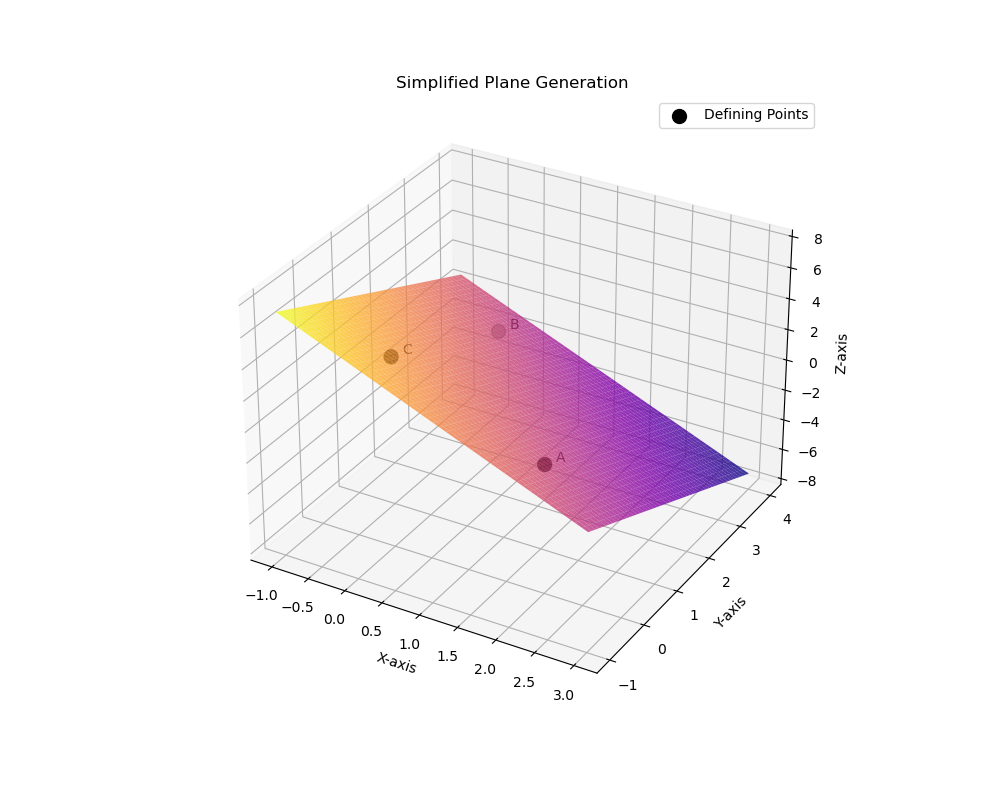
\includegraphics[width=0.9\columnwidth]{figs/plane.png}
    \caption{plane}
    \label{fig:placeholder_1}
\end{figure}
\end{document}